\documentclass[12pt, a4paper]{report}

\usepackage{amsmath,amsthm,amssymb}
\usepackage{mathtext}
\usepackage[T1,T2A]{fontenc}
\usepackage[utf8]{inputenc}
\usepackage[english,russian]{babel}
\usepackage{listings}
\usepackage{graphicx}
\usepackage{tablefootnote}
\usepackage{indentfirst}
\usepackage{color}
\usepackage{float}
\usepackage{caption}
\captionsetup[table]{singlelinecheck=off}
\captionsetup[lstlisting]{singlelinecheck=off, labelformat=empty}
\usepackage{pgfplots}
\pgfplotsset{compat=1.9}
\usepackage[left=3cm,right=1cm, top=2cm,bottom=2cm,bindingoffset=0cm]{geometry}
\graphicspath{{./img/}}

\lstset{ 
  backgroundcolor=\color{white},   % choose the background color; you must add \usepackage{color} or \usepackage{xcolor}; should come as last argument
  breaklines=true,                 % sets automatic line breaking
  captionpos=t,                    % sets the caption-position to bottom
  commentstyle=\color{green},    % comment style
  keywordstyle=\color{blue},       % keyword style
  language=C++,                 % the language of the code
  numbers=left,                    % where to put the line-numbers; possible values are (none, left, right)
  numbersep=5pt,                   % how far the line-numbers are from the code
  numberstyle=\tiny\color{black}, % the style that is used for the line-numbers
  showspaces=false,                % show spaces everywhere adding particular underscores; it overrides 'showstringspaces'
  showstringspaces=false,          % underline spaces within strings only
  showtabs=false,                  % show tabs within strings adding particular underscores
  stepnumber=1,                    % the step between two line-numbers. If it's 1, each line will be numbered
  stringstyle=\color{yellow},     % string literal style
  tabsize=2,	                   % sets default tabsize to 2 spaces
  frame=single
}

\begin{document}

\begin{titlepage}
	\noindent \begin{minipage}{0.15\textwidth}
	
\includegraphics[width=\linewidth]{bauman_image}
	\end{minipage}
	\footnotesize\noindent \begin{minipage}{0.8\textwidth}\centering
		\textbf{Министерство науки и высшего образования Российской Федерации}\\
		\textbf{Федеральное государственное бюджетное образовательное учреждение}\\
		\textbf{высшего образования}\\
		\textbf{~~~«Московский государственный технический университет}\\
		\textbf{имени Н.Э.~Баумана}\\
		\textbf{(национальный исследовательский университет)»}\\
		\textbf{(МГТУ им. Н.Э.~Баумана)}
	\end{minipage}
	
	\noindent\rule{17cm}{3pt}
	\newline\newline
	\large\noindent ФАКУЛЬТЕТ $\underline{\text{Информатика и системы управления}}$ \newline\newline
	\noindent КАФЕДРА $\underline{\text{Программное обеспечение ЭВМ и информационные технологии}}$\newline\newline\newline\newline\newline
	
	
	\begin{center}
		\noindent
			\LARGE\textbf{Отчёт по лабораторной работе №4}\newline
			\textbf{по дисциплине "Анализ алгоритмов"}\newline\newline
	\end{center}
	
	\large\noindent\textbf{Тема} $\underline{\text{Параллельный алгоритм сортировки слиянием}}$\newline\newline
	\noindent\textbf{Студент} $\underline{\text{Жабин Д.В.}}$\newline\newline
	\noindent\textbf{Группа} $\underline{\text{ИУ7-54Б}}$\newline\newline
	\noindent\textbf{Преподаватель} $\underline{\text{Волкова Л.Л.}}$\newline\newline\newline
	
	\begin{center}
		\large\vfill
		Москва, 2021 г.
	\end{center}
\end{titlepage}

\setlength{\parindent}{1.25cm}

\setcounter{page}{2}\large\linespread{1.3}\tableofcontents

\newpage
\chapter*{Введение}
\addcontentsline{toc}{chapter}{Введение}

Современная архитектура электронно-вычислительных машин позволяет работать с параллелизмом. Параллелизм~--- это свойство систем, при котором несколько вычислений выполняются одновременно и при этом, возможно, взаимодействуют друг с другом. Вычисления могут выполняться на нескольких ядрах одного чипа с вытесняющим разделением времени потоков на одном процессоре, либо выполняться на физически отдельных процессорах. Для выполнения параллельных вычислений разработан ряд математических моделей, в том числе сети Петри, исчисление процессов, модели параллельных случайных доступов к вычислениям и модели акторов.

Многие языки программирования дают возможность работать с потоками. Потоки~--- абстракция операционной системы, позволяющая выполнять части кода параллельно. Каждый поток имеет \verb|контекст|, в который входит участок памяти под стек и копию регистров процессора. Потоков в системе может быть запущено куда больше, чем имеется процессоров и ядер, поэтому операционная система занимается диспетчеризацией и планированием выполнения процессов, восстанавливая регистры в ядрах процессора для работы некоторого потока некоторое время, затем сохраняет обратно и даёт выполняться следующему. 

Потоки можно погружать в сон на некоторое время, а также разделять один и тот же участок памяти компьютера между потоками.

Так, работа с потоками позволит в разы увеличить производительность того или иного алгоритма.

Целью лабораторной работы является исследование возможностей параллельных вычислений в системе. Для её достижения поставлены следующие задачи:

\begin{itemize}
	\item выбрать стандартный алгоритм, производящий вычисления или работающий с памятью;
	\item изучить его и оценить возможность распараллеливания с целью увеличения производительности;
	\item разработать схемы обоих алгоритмов;
	\item реализовать изученные алгоритмы;
	\item провести тестирование реализаций алгоритмов;
	\item провести сравнительный анализ скорости работы реализаций алгоритмов с учетом возможности выделения разного количества потоков.
\end{itemize}

\newpage
\chapter*{1 Аналитическая часть}
\addcontentsline{toc}{chapter}{1 Аналитическая часть}

Рассмотрим стандартный алгоритм сортировки массива слиянием, который в дальнейшем будет распараллелен.

\section*{1.1 Стандартный алгоритм сортировки слиянием}
\addcontentsline{toc}{section}{1.1 Стандартный алгоритм сортировки слиянием}

Стандартный алгоритм сортировки слиянием [4] описывает стратегию\newline \verb|Разделяй и властвуй|.

При использовании этой стратегии основная задача делится на подзадачи. Когда решение для каждой подзадачи готово, их результаты объединяются для решения основной задачи.

Пусть, необходимо отсортировать массив $array$. Подзадача состоит в том, чтобы отсортировать часть этого массива, начиная с индекса $begin$ и заканчивая индексом $end$, обозначенную как $array[begin..end]$.\newline

\textbf{Разделяй}

Если $point$ является промежуточной точкой между $begin$ и $end$, то можно разбить массив $array[begin..end]$ на два подмассива $subarray[begin..point]$ и $subarray[point + 1..end]$.\newline

\textbf{Влавствуй}

На это этапе происходит попытка отсортировать оба подмассива\newline $subarray[begin..point]$ и $subarray[point + 1..end]$. Если еще не достигнут базовый вариант (размер подмассива меньше 2), можно снова разбить каждый подмассив и попытаться отсортировать их.\newline

\textbf{Комбинируй}

Когда достигается базовый вариант, получается два отсортированных подмассива $subarray[begin..point]$ и $subarray[point + 1..end]$ для массива\newline $array[begin..end]$. Результаты объединяются, создавая отсортированный массив $array[begin..end]$ из двух отсортированных подмассивов.\newline

Стандартный алгоритм сортировки слиянием реализует вышеописанную стратегию \verb|Разделяй и властвуй|. На рисунке (1.1) приведен пример работы этого алгоритма.

\begin{figure}[H]
\center{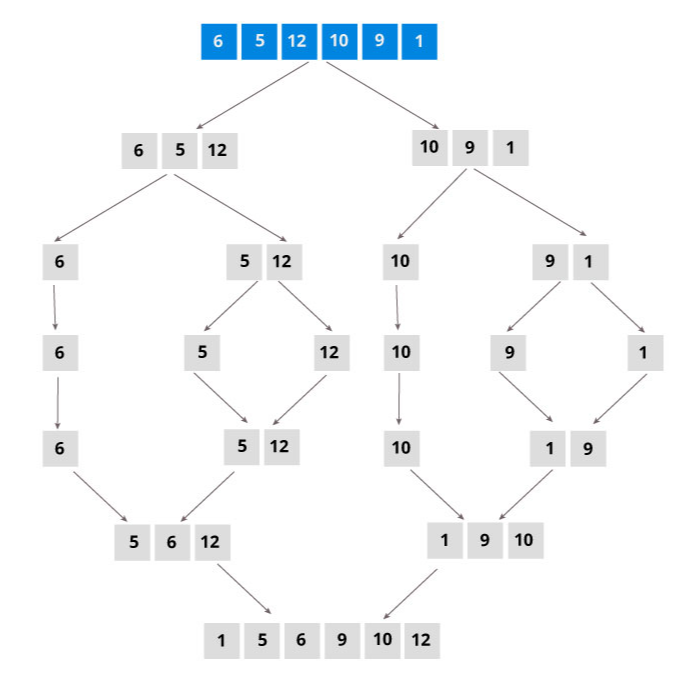
\includegraphics[scale=0.72]{exampleMergeSort.jpg}}
\caption*{Рисунок 1.1~--- Пример работы стандартного алгоритма сортировки слиянием}
\end{figure}

\section*{1.2 Вывод по аналитической части}
\addcontentsline{toc}{section}{1.2 Вывод по аналитической части}
В данном разделе был рассмотрен стандартный алгоритм сортировки слиянием. Можно заметить, что алгоритм допускает естественное распараллеливание.\newline

\newpage
\chapter*{2 Конструкторская часть}
\addcontentsline{toc}{chapter}{2 Конструкторская часть}

На основе полученных аналитических данных распараллелим стандартный алгоритм сортировки слиянием и построим схемы обоих алгоритмов.

\section*{2.1 Параллельная сортировка слиянием}
\addcontentsline{toc}{section}{2.1 Параллельная сортировка слиянием}

Легко заметить, что массив при каждом рекурсивном вызове делится на две примерно равные части и производится сортировка сначала левой, а затем правой частей массива. Это, значит что последовательные действия можно заменить на параллельные. При каждом рекурсивном вызове будет создаваться поток, который займется сортировкой левой части исходного массива в то время, как вызвавший его поток будет сортировать правую часть. Таким образом можно добиться максимального количества параллельно работающих потоков. При такой реализации каждый поток будет работать только с вверенной ему частью исходного массива, то есть не возникнет проблем, связанных с множественным доступом к данным.

Поскольку на реальной вычислительной машине невозможно добиться создания бесконечного количества потоков, нужно отслеживать текущий уровень иерархии рекурсивных вызовов для своевременного прекращения создания потоков. При достижении максимально возможного количества созданных потоков каждый из них будет параллельно выполнять стандартный алгоритм сортировки слиянием.

\section*{2.2 Схемы алгоритмов}
\addcontentsline{toc}{section}{2.2 Схемы алгоритмов}
На рисунках 2.1--2.4 представлены схемы алгоритмов сортировки слиянием.

\begin{figure}[H]
\center{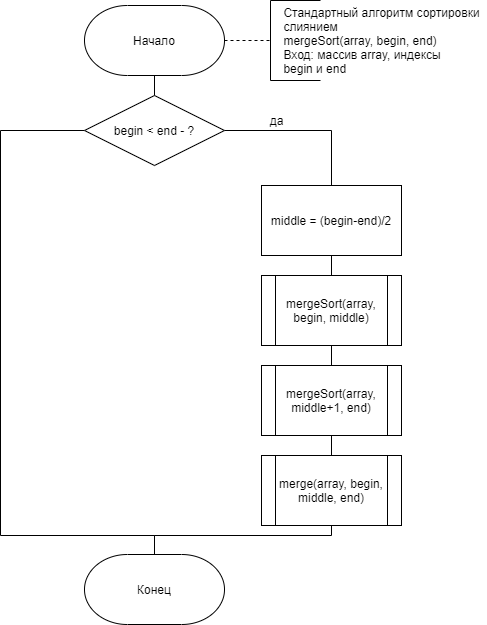
\includegraphics[scale=0.72]{simplesort.png}}
\caption*{Рисунок 2.1~--- Стандартный алгоритм сортировки слиянием}
\end{figure}

\begin{figure}[H]
\center{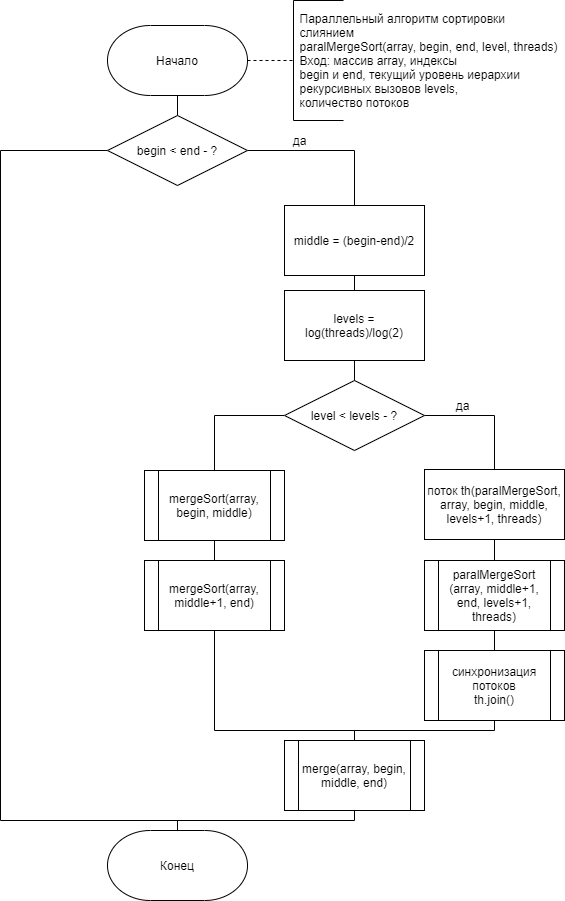
\includegraphics[scale=0.72]{parsort.png}}
\caption*{Рисунок 2.2~--- Параллельная сортировка слиянием}
\end{figure}

\begin{figure}[H]
\center{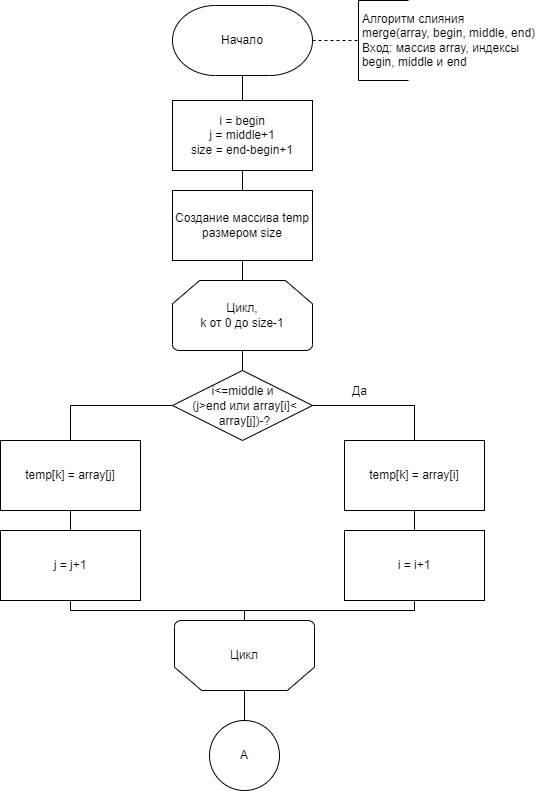
\includegraphics[scale=0.72]{merge1.png}}
\caption*{Рисунок 2.3~--- Алгоритм слияния. Часть 1}
\end{figure}

\begin{figure}[H]
\center{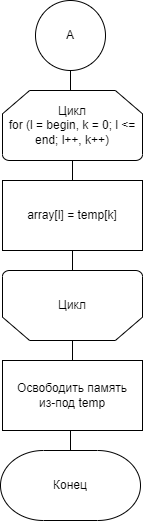
\includegraphics[scale=0.72]{merge2.png}}
\caption*{Рисунок 2.4~--- Алгоритм слияния. Часть 2}
\end{figure}

\section*{2.3 Типы и структуры данных}
\addcontentsline{toc}{section}{2.3 Типы и структуры данных}

Для хранения исходного набора значений используется массив целых чисел. Запись результата будет производиться в исходный массив. Каждый поток будет работать только со своей частью исходного массива, таким образом избегается возможность критических ситуаций и потери информации.

\section*{2.4 Способ тестирования}
\addcontentsline{toc}{section}{2.4 Способ тестирования}

Реализуемое программное обеспечение будет протестировано методом \verb|черного ящика|. Для тестирования были выделены следующие классы эквивалентности:
\begin{enumerate}
	\item Неверный выбор режима работы программы~--- пустой ввод, нецифровой символ.
	\item Верный выбор режима работы программы~--- цифра из диапазона $[1..3]$ или число, выходящее за пределы указанного диапазона.
	\item Неверный выбор количества потоков при параллельной сортировке~--- пустой ввод, нецифровой символ или число, не входящее в набор указанных доступных значений.
	\item Верный выбор количества потоков при параллельной сортировке~--- число из набора $(2, 4, 8, 16)$.
	\item Неверный ввод размера исходного массива~--- пустой ввод, нецифровой символ или целое неположительное или вещественное число.
	\item Верный ввод размера исходного массива~--- целое положительное число.
	\item Неверный ввод элемента исходного массива~--- пустой ввод, нецифровой символ или вещественное число.
	\item Верный ввод элемента исходного массива~--- целое число.
\end{enumerate}

\section*{2.5 Тестовые данные}
\addcontentsline{toc}{section}{2.5 Тестовые данные}

В таблицах 2.1--2.4 представлены тестовые данные.

\begin{table} [H]
	\caption*{Таблица 2.1~--- Функциональные тесты выбора режима работы программы}
	\begin{tabular}[l]{|c c c|}
		\hline
		Номер тестового случая & Ввод & Ожидаемый результат  \\
 
		1 & \verb|_|\tablefootnote[1]{Пустой ввод} & Неверный ввод \\\hline 

		2 & $\alpha$ & Неверный ввод \\\hline 

		3 & 1 & Введите размер массива \\\hline 

		4 & 2 & Введите количество потоков \\\hline 

		5 & 3 & Таблица замеров времени \\\hline
	\end{tabular}
\end{table}

\begin{table} [H]
	\caption*{Таблица 2.2~--- Функциональные тесты выбора количества потоков}
	\begin{tabular}[l]{|c c c|}
		\hline
		Номер тестового случая & Ввод & Ожидаемый результат  \\

		1 & $\verb|_|^1$ & Неверный ввод \\\hline 

		2 & $\alpha$ & Неверный ввод \\\hline 

		3 & 1 & Неверный ввод \\\hline 

		4 & 2 & Введите размер массива \\\hline
	\end{tabular}
\end{table}

\begin{table} [H]
	\caption*{Таблица 2.3~--- Функциональные тесты ввода размера исходного массива}
	\begin{tabular}[l]{|c c c|}
		\hline
		Номер тестового случая & Ввод & Ожидаемый результат  \\

		1 & $\verb|_|$\tablefootnote{Пустой ввод} & Неверный ввод \\\hline 

		2 & $\alpha$ & Неверный ввод \\\hline 

		3 & 0 & Неверный ввод \\\hline 

		4 & 2.2 & Неверный ввод \\\hline
		
		5 & 2 & Введите элементы массива \\\hline
	\end{tabular}
\end{table}

\begin{table} [H]
	\caption*{Таблица 2.4~--- Функциональные тесты ввода элементов исходного массива}
	\begin{tabular}[l]{|c c c|}
		\hline
		Номер тестового случая & Ввод & Ожидаемый результат  \\

		1 & $\verb|_|^1$ & Неверный ввод \\\hline 

		2 & $\alpha$ & Неверный ввод \\\hline 

		3 & 2.2 & Неверный ввод \\\hline
		
		4 & 0 & $...$\tablefootnote[2]{Ожидание ввода следующего элемента} \\\hline 
	\end{tabular}
\end{table}

\section*{2.6 Структура программного обеспечения}
\addcontentsline{toc}{section}{2.6 Структура программного обеспечения}

Программное обеспечение разработано с использованием структурного подхода, поскольку использование объектов в данном случае не дает преимуществ. Программа содержит функцию \verb|mergeSort|, принимающая на вход указатель на исходный массив, индекс начала и индекс конца обрабатываемой части массива. Она реализует стандартный алгоритм сортировки слиянием. Функция \verb|merge| реализует слияние двух отсортированных частей массива в один отсортированный. На вход она принимает указатель на исходный массив, индекс начала и конца сливаемой части массива, а также индекс конца первого подмассива. Функция \verb|paralMergeSort| принимает те же параметры, что и функция \verb|mergeSort|, а также максимальное количество создаваемых потоков и текущий уровень иерархии рекурсивных вызовов. Все три функции ничего не возвращают, они лишь изменяют вверенные им части исходного массива. 

\section*{2.7 Вывод по конструкторской части}
\addcontentsline{toc}{section}{2.7 Вывод по конструкторской части}

Были разработаны схемы стандартного алгоритма сортировки слиянием и его распараллеленного аналога, а также подготовлены данные для тестирования программного обеспечения. 

\chapter*{3 Технологическая часть}
\addcontentsline{toc}{chapter}{3 Технологическая часть}

В данном разделе приведены средства реализации и листинги кода.

\section*{3.1 Требования к ПО}
\addcontentsline{toc}{section}{3.1 Требования к ПО}

К программе предъявляется ряд требований:

\begin{itemize}
	\item требования ко вводу
	\begin{itemize}
		\item должен быть выбран режим работы программы (целое число в дапазоне $[1..3]$);
		\item должны быть введены следующие значения: количество потоков при необходимости (целое число из набора $(2, 4, 8, 16)$), размер массива (целое положительное число), элементы массива (целые числа).
	\end{itemize}
	\item требования к выводу
	\begin{itemize}
		\item результат сортировки;
		\item таблица времен работы реализаций алгоритмов на случайных значениях при разных размерах массивов и разных количествах потоков в миллисекундах.
	\end{itemize}
	\item ограничения работы программы
	\begin{itemize}
		\item при вводе режима работы программы, выходящего за пределы указанного диапазона, программа завершает работу.
	\end{itemize}
	\item функциональные требования к программному обеспечиванию:
	\begin{itemize}
		\item при запуске программа должна выводить меню с возможными режимами работы;
		\item программа должна сортировать входной массив целых чисел стандартным алгоритмом сортировки слиянием или его распараллеленным аналогом;
		\item в исследовательском режиме программа должна замерять время выполнения реализаций стандартного алгоритма сортировки слиянием и его распараллеленного аналога при различных размерах массивов и с разным количеством используемых потоков в последнем случае.
	\end{itemize}
\end{itemize}

\section*{3.2 Средства реализации}
\addcontentsline{toc}{section}{3.2 Средства реализации}

Для реализации ПО был выбран язык программирования \verb|С++| [1]. Это обусловлено наличием широкого спектра возможностей для работы с потоками и распараллеливания алгоритмов. 

В качестве среды разработки была выбрана \verb|Visual Studio Code| [3]. Достаточный опыт работы в этой среде, удобства написания кода и его автодополнения стали ключевыми при выборе.

\section*{3.3 Реализация алгоритмов}
\addcontentsline{toc}{section}{3.3 Реализация алгоритмов}

В листингах 3.1 - 3.3 приведена реализация рассматриваемых алгоритмов.

\newpage
\begin{lstlisting}[title=Листинг 3.1~--- Стандартный алгоритм сортировки слиянием]
void mergeSort(int *array, int begin, int end) {
    if (begin < end) {
        int middle = (end + begin) / 2;
        mergeSort(array, begin, middle);
        mergeSort(array, middle+1, end);
        merge(array, begin, middle, end);
    }
}
\end{lstlisting}

\begin{lstlisting}[title=Листинг 3.2~--- Параллельная сортировка слиянием]
void paralMergeSort(int *array, int begin, int end, int level, int threads) {
    if (begin < end) {
        int middle = (end + begin) / 2;
        int levels = (int)(log(((double)threads) / log(2.0)));
        if (level < levels) {
            thread th(paralMergeSort, array, begin,
            	middle, level+1, threads);
            paralMergeSort(array, middle+1, end, level+1, threads);
            th.join();
        } else {
            mergeSort(array, begin, middle);
            mergeSort(array, middle+1, end);
        }
        merge(array, begin, middle, end);
    }
}
\end{lstlisting}

\newpage
\begin{lstlisting}[title=Листинг 3.3~--- Функция слияния двух отсортированных массивов]
void merge(int *array, int begin, int middle, int end) {
    int i = begin, j = middle + 1, size = end - begin + 1;
    int *temp = (int *)malloc(sizeof(int)*size);
    for (int k = 0; k < size; k++) {
        if (i <= middle &&
           (j > end || array[i] < array[j])) {
            temp[k]=array[i];
            i++;
        } else {
            temp[k]=array[j];
            j++;
        }
    }
    for (int l = begin, k = 0; l <= end; l++, k++) {
        array[l] = temp[k];
    }
    free(temp);
}
\end{lstlisting}

\section*{3.4 Вывод по технологической части}
\addcontentsline{toc}{section}{3.4 Вывод по технологической части}

В данном разделе были реализованы стандартный алгоритм сортировки слиянием и его распараллеленный аналог.

\chapter*{4 Исследовательская часть}
\addcontentsline{toc}{chapter}{4 Исследовательская часть}

В этом разделе будет исследовано быстродействие разработанных реализаций алгоритмов.

\section*{4.1 Технические характеристики}
\addcontentsline{toc}{section}{4.1 Технические характеристики}

Ниже приведены технические характеристики устройства, на котором было проведено тестирование ПО:

\begin{itemize}
	\item операционная система Windows 10 64-разрядная;
	\item оперативная память 16 ГБ;
	\item процессор Intel(R) Core(TM) i5-4690 @ 3.50ГГц.
\end{itemize}

\section*{4.2 Время выполнения реализаций алгоритмов}
\addcontentsline{toc}{section}{4.2 Время выполнения реализаций алгоритмов}

Чтобы точно оценить время выполнения реализаций алгоритмов была использована функция \verb|std::chrono::high_resolution_clock::now()| [2], которая возвращает точку, указывающую на текущее время. Так, с помощью двух последовательных вызовов можно определить, в течение какого времени выполнялась функция.

В таблицe 4.1 и на графике 4.1 показаны результаты замеров.

\begin{table} [H]
	\caption*{Таблица 4.1~--- Зависимость времени выполнения реализаций алгоритмов сортировки слиянием от размера массива (в миллисекундах)}
	\begin{tabular}[l]{|c c c c c c|}
		\hline
		Размер массива & Стандарт\tablefootnote[1]{Стандартный алгоритм сортировки слиянием} & 2 потока\tablefootnote[2]{Параллельная сортировка слиянием с 2 потоками} & 4 потока\tablefootnote[3]{Параллельная сортировка слиянием с 4 потоками} & 8 потоков\tablefootnote[4]{Параллельная сортировка слиянием с 8 потоками} & 16 потоков\tablefootnote[5]{Параллельная сортировка слиянием с 16 потоками}  \\

		1000 & 0.310042 & 0.328200 & 0.327511 & 0.361685 & 0.492158 \\\hline 

		5000 & 1.350680 & 0.964878 & 0.874131 & 0.761405 & 0.778045 \\\hline 

		10000 & 1.468820 & 0.914586 & 0.820653 & 0.745670 & 0.777463 \\\hline 

		100000 & 13.208900 & 7.088850 & 7.042640 & 5.179420 & 4.749100 \\\hline 
		
		200000 & 27.689400 & 14.715900 & 14.693300 & 10.069600 & 8.754370 \\\hline 

		500000 & 74.242100 & 39.297600 & 39.188600 & 24.013900 & 22.259800 \\\hline 

		1000000 & 156.021000 & 82.423000 & 82.253000 & 49.909500 & 44.313600 \\\hline
	\end{tabular}
\end{table}

\begin{figure}[H]
\caption*{График 4.1~--- Время выполнения реализаций алгоритмов сортировки слиянием}
\begin{center}
\begin{tikzpicture}
\begin{axis}[
	xlabel = {$\text{Размер массива}$},
	ylabel = {$\text{Время, мс}$},
	legend pos = north west,
	height = 0.6\paperheight, 
	width = 0.75\paperwidth,
	xmin = 0,
	xmax = 10^6+1000,
	ymin = 0,
]
\legend{ 
	$\text{Стандартный алгоритм сортировки слиянием}$, 
	$\text{2-поточный алгоритм сортировки слиянием}$,
	$\text{4-поточный алгоритм сортировки слиянием}$,
	$\text{8-поточный алгоритм сортировки слиянием}$,
	$\text{16-поточный алгоритм сортировки слиянием}$
};
\addplot coordinates {
	(1000,0.310042) (5000,1.350680) (10000,1.468820) (100000,13.208900) (200000,27.689400) (500000,74.242100) (1000000,156.021000)
};
\addplot coordinates {
	(1000,0.328200) (5000,0.964878) (10000,0.914586) (100000,7.088850) (200000,14.715900) (500000,39.297600) (1000000,82.423000)
};
\addplot coordinates {
	(1000,0.327511) (5000,0.874131) (10000,0.820653) (100000,7.042640) (200000,14.693300) (500000,39.188600) (1000000,82.253000)
};
\addplot coordinates {
	(1000,0.361685) (5000,0.761405) (10000,0.74567) (100000,5.17942) (200000,10.0696) (500000,24.0139) (1000000,49.9095)
};
\addplot coordinates {
	(1000,0.492158) (5000,0.778045) (10000,0.777463) (100000,4.7491) (200000,8.75437) (500000,22.2598) (1000000,44.3136)
};
\end{axis}
\end{tikzpicture}
\end{center}
\end{figure}

\section*{4.3 Вывод по исследовательской части}
\addcontentsline{toc}{section}{4.3 Вывод по исследовательской части}

По результатам замеров можно сказать, что на массивах больших размеров многопоточный алгоритм в несколько раз быстрее, чем стандартный. Но на малых размерах (до 1000 элементов) стандартный работает быстрее, поскольку задача для каждого потока оказывается настолько простой, что намного больше времени уходит на создание самих потоков.


\chapter*{Заключение}
\addcontentsline{toc}{chapter}{Заключение}

В ходе проделанной работы была достигнута поставленная цель и решены следующие задачи:

\begin{itemize}
	\item выбран и изучен стандартный алгоритм, работающий с памятью;
	\item разработаны схемы стандартного алгоритма и его распараллеленной версии;
	\item реализованы эти алгоритмы;
	\item проведено тестирование реализаций алгоритмов;
	\item проведен сравнительный анализ скорости работы реализаций алгоритмов с учетом возможности выделения разного количества потоков.
\end{itemize}

Было доказано, что имеет смысл выделять потоки только в том случае, если каждому потоку будет дана сложная задача, в противном случае намного больше времени будет затрачиваться на создание потоков.

\chapter*{Литература}
\addcontentsline{toc}{chapter}{Литература}

[1] C++ [Электронный ресурс]. Режим доступа: https://isocpp.org/. Дата обращения: 11.11.2021.\\

[2] Функция now() [Электронный ресурс]. Режим доступа: \newline https://en.cppreference.com/w/cpp/chrono/high-resolution-clock/now. Дата обращения: 11.11.2021.\\

[3] Visual Studio Code - Code Editing [Электронный ресурс]. Режим доступа: https://code.visualstudio.com. Дата обращения: 11.11.2021.\\

[4] Сортировки [Электронный ресурс]. Режим доступа: \newline https://function-x.ru/cpp-algoritmy-sortirovki.html. Дата обращения: 11.11.2021.

\end{document}